% Options for packages loaded elsewhere
\PassOptionsToPackage{unicode}{hyperref}
\PassOptionsToPackage{hyphens}{url}
%
\documentclass[
]{article}
\usepackage{lmodern}
\usepackage{amssymb,amsmath}
\usepackage{ifxetex,ifluatex}
\ifnum 0\ifxetex 1\fi\ifluatex 1\fi=0 % if pdftex
  \usepackage[T1]{fontenc}
  \usepackage[utf8]{inputenc}
  \usepackage{textcomp} % provide euro and other symbols
\else % if luatex or xetex
  \usepackage{unicode-math}
  \defaultfontfeatures{Scale=MatchLowercase}
  \defaultfontfeatures[\rmfamily]{Ligatures=TeX,Scale=1}
\fi
% Use upquote if available, for straight quotes in verbatim environments
\IfFileExists{upquote.sty}{\usepackage{upquote}}{}
\IfFileExists{microtype.sty}{% use microtype if available
  \usepackage[]{microtype}
  \UseMicrotypeSet[protrusion]{basicmath} % disable protrusion for tt fonts
}{}
\makeatletter
\@ifundefined{KOMAClassName}{% if non-KOMA class
  \IfFileExists{parskip.sty}{%
    \usepackage{parskip}
  }{% else
    \setlength{\parindent}{0pt}
    \setlength{\parskip}{6pt plus 2pt minus 1pt}}
}{% if KOMA class
  \KOMAoptions{parskip=half}}
\makeatother
\usepackage{xcolor}
\IfFileExists{xurl.sty}{\usepackage{xurl}}{} % add URL line breaks if available
\IfFileExists{bookmark.sty}{\usepackage{bookmark}}{\usepackage{hyperref}}
\hypersetup{
  pdftitle={Analyzing SARS-CoV-2 in Pennsylvania Wastewater Samples},
  pdfauthor={Alyssa Ramirez},
  hidelinks,
  pdfcreator={LaTeX via pandoc}}
\urlstyle{same} % disable monospaced font for URLs
\usepackage[margin=1in]{geometry}
\usepackage{longtable,booktabs}
% Correct order of tables after \paragraph or \subparagraph
\usepackage{etoolbox}
\makeatletter
\patchcmd\longtable{\par}{\if@noskipsec\mbox{}\fi\par}{}{}
\makeatother
% Allow footnotes in longtable head/foot
\IfFileExists{footnotehyper.sty}{\usepackage{footnotehyper}}{\usepackage{footnote}}
\makesavenoteenv{longtable}
\usepackage{graphicx,grffile}
\makeatletter
\def\maxwidth{\ifdim\Gin@nat@width>\linewidth\linewidth\else\Gin@nat@width\fi}
\def\maxheight{\ifdim\Gin@nat@height>\textheight\textheight\else\Gin@nat@height\fi}
\makeatother
% Scale images if necessary, so that they will not overflow the page
% margins by default, and it is still possible to overwrite the defaults
% using explicit options in \includegraphics[width, height, ...]{}
\setkeys{Gin}{width=\maxwidth,height=\maxheight,keepaspectratio}
% Set default figure placement to htbp
\makeatletter
\def\fps@figure{htbp}
\makeatother
\setlength{\emergencystretch}{3em} % prevent overfull lines
\providecommand{\tightlist}{%
  \setlength{\itemsep}{0pt}\setlength{\parskip}{0pt}}
\setcounter{secnumdepth}{-\maxdimen} % remove section numbering

\title{Analyzing SARS-CoV-2 in Pennsylvania Wastewater Samples}
\author{Alyssa Ramirez}
\date{13 December, 2024}

\begin{document}
\maketitle

\hypertarget{background-and-overview}{%
\section{Background and Overview}\label{background-and-overview}}

The monitoring and detection of SARS-CoV-2 RNA in wastewater has emerged
as another tool in aiding the surveillance of SARS-CoV-2 in populations.
Wastewater surveillance provides non-invasive, cost-effective methods
for insights and trends in the spread in SARS-CoV-2 RNA within a region.
This approach has been useful in understanding hot spots, strain
development, drift in other regions and overall helpful insights to the
public health. Wastewater surveillance has been proven to be efficient
in identifying patterns of viral transmission, monitoring genetic drift,
and supporting epidemiological studies.(Peccia \emph{et al.}, 2022) This
study utilizes Pennsylvania wastewater surveillance systems (PAWSS)
data, a statewide surveillance system that collects waste samples in
diverse communities. Data from this study were collected from multiple
collection sites: wastewater treatment facilities (WWTFs), individual,
buildings or congregate settings, correctional facilities, dormitories,
long-term care facilities and schools.(Pennsylvania Department of
Health, 2024) The data focuses on population sizes, sequencing
information, temporal trends and waste water sample collecting methods.
Wastewater surveillance is specifically effective for identifying
SARS-CoV-2 viral RNA, including non-traditional cases that could
potentially go unnoticed by clinical testing. These also include even
asymptomatic and oligosymptomatic samples. Wastewater surveillance
offers a specific advantage over traditional clinical testing by using
large-scale monitoring of SARS-CoV-2 RNA with minimal resources. As
stated, this approach ``only needs to test one sample for mass screening
of SARS-CoV-2. Clinical testing, on the other hand, may require 10,000
individual tests and bears the associated costs for sample collection
and investments in high-throughput infrastructure'' (Peccia \emph{et
al.}, 2022) This highlights the cost-effectiveness and efficiency of
wastewater surveillance as a whole. This study focuses on the essential
factors that influence the reliability and effectiveness of wastewater
surveillance, including sampling methods, population size, and temporal
trends. Sampling methods, such as composite and grab sampling. These
methods differ in their ability to provide viral RNA signals. Inspecting
population size impacts the concentration of viral RNA and the potential
risk of diluting detectable viral RNA in larger populations. On the
other hand, temporal trends reveal how SARS-CoV-2 RNA levels can vary
overtime and how population dynamics influence viral community infection
rates. Bash and Rstudio technologies were used to create visual
representations of data.

\hypertarget{research-question}{%
\section{Research Question}\label{research-question}}

The primary aim of this study is to investigate how sampling methods
(composite vs.~grab), collection periods, and population size influence
the detection and reliability of SARS-CoV-2 RNA in wastewater. By
analyzing sequencing metadata, this research seeks to uncover factors
that impact viral RNA detection, with implications for improving public
health surveillance systems.

\hypertarget{methods}{%
\section{Methods}\label{methods}}

\hypertarget{wastewater-data-collection}{%
\paragraph{Wastewater data
collection}\label{wastewater-data-collection}}

Wastewater samples were collected from various locations across
Pennsylvania from the Pennsylvania Wastewater Surveillance System
(PAWSS). Samples were gathered used 2 types of filtering mechanisms,
composite and grab sampling methods. Composite samples were collected
over a duration of 24 hours and considered a ``average'' of waste.
Compared to grab sampling, which is a one-time sample.(Kmush \emph{et
al.}, 2022)

\hypertarget{rna-purification-and-sequencing}{%
\paragraph{RNA Purification and
Sequencing}\label{rna-purification-and-sequencing}}

Following extraction from composite and grab samplings, reverse
transcription to synthesize complementary DNA (cDNA) is used on the
purified RNA. The purified RNA is synthesized using Reverse
Transcription Polymerase Chain Reaction (RT-PCR). The cDNA is amplified
and prepared for sequencing using the Illumina COVIDSeq™ Assay, which
targets the SARS-CoV-2 genome, including ``regions prone to single
nucleotide polymorphisms (SNPs).''Sequencing was performed on an
Illumina platform, generating high-throughput data with robust coverage
of genomic regions of interest."(Surveillance of infectious disease
through wastewater sequencing: Detect sars-cov-2 variants and other
respiratory viruses in the community, 2024) To eliminate contaminants
and ensure accurate data, quality control metrics were applied to
sequencing reads. The sequencing metadata were obtained from the
National Library of Medicine BioProject database (Accession:
PRJNA1039783), submitted by the Pennsylvania Department of Health Bureau
of Laboratories.(Health Bureau of Laboratories Submission Group, 2023)

\hypertarget{data-processing-and-analysis}{%
\paragraph{Data Processing and
Analysis}\label{data-processing-and-analysis}}

Sequencing data were processed using a bioinformatics makefile pipeline,
designed to analyze the genomic metadata. GFF annotation files and VCF
datasets were utilized to identify SNPs and functional data. The
pipeline consisted of the following key steps: 1.GFF Annotation Parsing:
The genomic feature file (GFF) was read and parsed to extract gene
annotations, enabling identification of specific SARS-CoV-2 genomic
regions.{[}2023Djaffardjy{]} 2.Gene Extraction: Relevant genomic
features were filtered to produce a table of gene names and coordinates
for downstream analyses.{[}2023Djaffardjy{]} 3.VCF File Integration:
Variant call format (VCF) files were parsed, cleaned, and merged with
metadata to create a unified dataset containing SNP-level information
for all samples.{[}2023Djaffardjy{]} 4.SNP Annotation: SNPs were
annotated with gene information by merging the tidy VCF data with the
gene table and metadata.{[}2023Djaffardjy{]} The pipeline worked
effortlessly due to the \texttt{Bash} and \texttt{Rstudio} function
scripts previously provided by Professor Zimmerman, University of San
Francisco.

\hypertarget{data-visualization-and-statistical-analysis}{%
\paragraph{Data Visualization and Statistical
Analysis}\label{data-visualization-and-statistical-analysis}}

Visualizations and analyses were conducted using R programming. R
packages that were used are data manipulation are \texttt{ggplot2}
(Wickham, 2016), \texttt{dplyr} (Wickham \emph{et al.}, 2023) and
\texttt{tidyverse} (Wickham and others, 2023b). \texttt{Rmarkdown} was
used for report generation and rendering Markdown files into HTML and
pdf. (Xie and others, 2023) The R package \texttt{ggthemes}(Arnold,
2022) was used to create figures illustrating SNP distribution, temporal
trends, and relationships between key variables, such as population size
and RNA detection levels. To create color on the figures
\texttt{RColorBrewer}(Neuwirth, 2023) was used hand in hand with
\texttt{ggthemes}. The R package \texttt{magrittr} (Bache and Wickham,
2023) was used to utilize the pipe operator in code. To manipulate and
visualize variant call format (VCF) files, \texttt{vcfR}(Knaus and
others, 2023) was used. To enable report generation and integration of R
code \texttt{knitr} was used.(Xie, 2023) To make sure all of the
pipeline worked correctly \texttt{testthat} was used.(Wickham and
others, 2023a) Lastly, figures and tables were generated to summarize
and visualize the data. OpenAI's ChatGPT (OpenAI, 2024) was used to
create all figures and table.

\hypertarget{results}{%
\section{Results}\label{results}}

\hypertarget{impact-of-sampling-methods-on-viral-rna-detection}{%
\paragraph{Impact of Sampling Methods on Viral RNA
Detection}\label{impact-of-sampling-methods-on-viral-rna-detection}}

The analysis of composite and grab samples showed the distinct
differences in RNA detection consistency and data accuracy. Composite
samples, which were collected over the course of 24 hours, provided a
higher average in sequencing coverage compared to the grab
samples.(Kmush \emph{et al.}, 2022) As showed in \emph{Figure 5}, the
distribution of sampling methods showed a drastic difference in count.
Composite sampling minimizes temporal variability which results in a
overall higher value in representative number of SARS-CoV-2 RNA levels.
On the other hand, grab samples collect more at a single time but show a
major deduction in sequencing coverage and high variability. Which is
likely due to the temporal fluctuations of viral RNA levels in
wastewater.(Kmush \emph{et al.}, 2022)

\hypertarget{summary-of-sequencing-coverage-by-sampling-method}{%
\paragraph{Summary of Sequencing Coverage by Sampling
Method}\label{summary-of-sequencing-coverage-by-sampling-method}}

Table 1 summarizes the sequencing coverage for different sampling
matrices and methods. Composite samples consistently outperformed grab
samples in sequencing coverage, reinforcing their reliability for
wastewater surveillance. This table is used to support \emph{figure 5},
the table provides a detailed statistical metric on sequencing coverage
for composite and grab sampling methods. While \emph{Figure 5} visible
demonstrates the distribution coverage, \emph{Table 1} highlights
quantitative differences.

\hypertarget{temporal-trends-in-sequencing-coverage}{%
\paragraph{Temporal Trends in Sequencing
Coverage}\label{temporal-trends-in-sequencing-coverage}}

Temporal fluctuations in sequencing coverage were observed across
Pennsylvania, as shown in \emph{Figure 2} peaks in the figure show
sequencing coverage corresponding to periods of increases viral
prevalence in the Pennsylvania region. This suggests that the alignment
with SARS-CoV-2 case surges are representative. This also highlights the
utilities of wastewater surveillance in real-time epidemiological
trends. Even though, some moths exhibited a lower coverage, which could
potentially explain reduced viral shedding or sample processing errors.

\hypertarget{population-size-and-rna-detection-levels}{%
\paragraph{Population Size and RNA Detection
Levels}\label{population-size-and-rna-detection-levels}}

The relationship between population size and overall RNA detection
levels is represented in \emph{Figure 3}. A positive correlation between
the two variables can suggest that larger population sizes contribute to
more consistent viral RNA in wastewater. However, the relationship is
complex and influenced by multiple factors. As stated, ``Although the
association between population size and viral RNA concentrations may be
driven by absolute number of COVID-19 cases, it is important to state
that RNA concentrations may also be affected independently. As
population size increases, sewage flow increases due to increased water
usage causing dilution of viral RNA.'' (Carrat \emph{et al.}, 2022) This
further supports what is seen in \emph{Figure.4}, where there is a small
negative correlation between population size and average sequencing read
lengths. These figures can support the idea that RNA fragmentation leads
to an increase in sample diversity. Which can be insufficdent in
producing accurate and reliable data while in a larger population size.

\hypertarget{genomic-variability-across-sars-cov-2-genes}{%
\paragraph{Genomic Variability Across SARS-CoV-2
Genes}\label{genomic-variability-across-sars-cov-2-genes}}

Genomic variability is seen in \emph{Figure 1}, this figure represents
each gene seen in the data associated with its SNP count. The figure has
revealed that there is variability across the SARS-CoV-2 genes but the S
gene prevailed over all other genes. This finding is consistent with the
critical role of the spike protein in viral infectivity and host
interaction, making it a hotspot for mutations. This observation aligns
with global studies on SARS-CoV-2 evolution, emphasizing the need for
continued surveillance of the S gene to monitor emerging
variants.(Larsen \emph{et al.}, 2022)

\hypertarget{variant-distributions-in-pennsylvania}{%
\paragraph{Variant Distributions in
Pennsylvania}\label{variant-distributions-in-pennsylvania}}

The distribution of reference and alternate genome variants in
\emph{Figure 6} show a predominance of thymine (T) as the most frequent
alternate genome nucleotide. This finding may reflect regional patterns
in viral evolution, further underscoring the importance of localized
genomic surveillance.

\hypertarget{discussionn}{%
\section{Discussionn}\label{discussionn}}

This study highlights the value and importance of wastewater
surveillance as a cost effective and non-invasive tool to monitor
SARS-CoV-2 prevalence within populations.By analyzing data from the
Pennsylvania Wastewater Surveillance System (PAWSS), we explored the
impact of sampling methods, temporal trends and population size on the
reliability of SARS-CoV-2 RNA detection. Population size and RNA
detection did not correlate and had a small role against RNA detection
showing trends that were not predicted before going through the data.
Although the population size data was not helpful to the overall study,
it was helpful in the visualization of the S genome, seen as the most
common in the population. Temporal trends indicated variation over time
in sequencing coverage that could possibly reflect changes in the
SARS-CoV-2 genome. Our findings proved the superiority of composite
sampling over grab sampling method and proved the superiority of
consistency with sequencing coverage. These results outline the need for
standardized sampling methods to increase data quality for wastewater
surveillance programs. Temporal trends in sequencing coverage aligned
with periods of increased SARS-CoV-2 prevalence. Which demonstrates a
tracking in epidemiological shifts.

\hypertarget{figures}{%
\section{Figures}\label{figures}}

\includegraphics{Report_files/figure-latex/barplot-SNP-gene-distribution-1.pdf}
\textbf{Figure 1}: Bar plot showing the number of single nucleotide
polymorphisms (SNPs) identified across different genes of SARS-CoV-2.
The genes are labeled on the x-axis, and the y-axis indicates the count
of SNPs.

\includegraphics{Report_files/figure-latex/figure-1,normalized-sequence-coverage-1.pdf}

\textbf{Figure 2}:Temporal Trends in Normalized Sequencing Coverage Over
Time in Pennsylvania The plot shows normalized sequencing coverage
(SARS-CoV-2 RNA levels per person) over time for wastewater samples
collected in Pennsylvania.

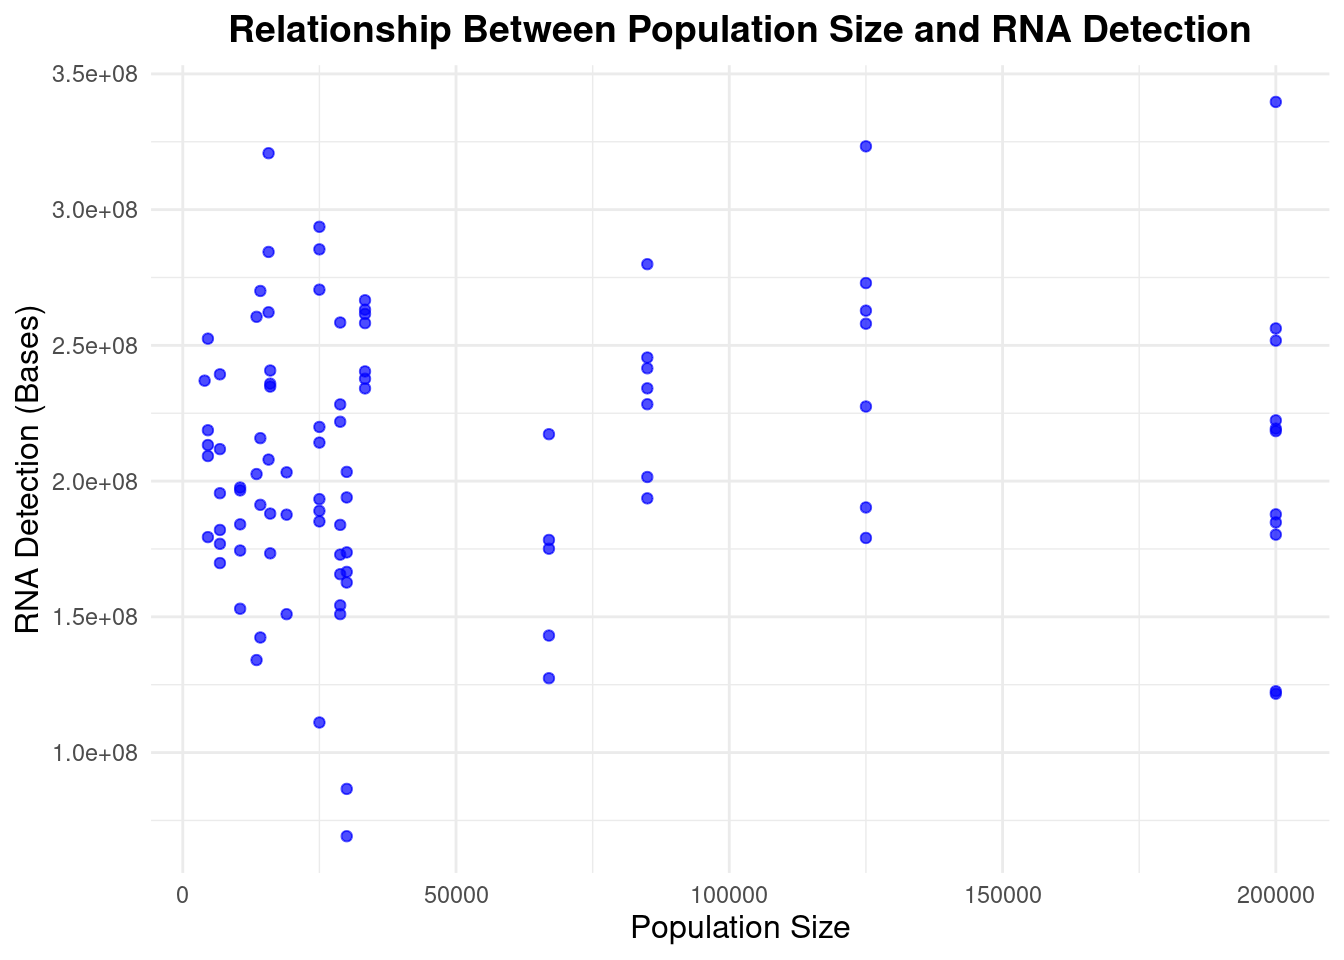
\includegraphics{Report_files/figure-latex/population-vs-rna-detection-1.pdf}

\textbf{Figure 3}:Scatter plot showing the relationship between
population size and RNA detection levels (measured as bases) in
wastewater samples. Each point represents a data sample, and the
distribution illustrates whether population size affects RNA detection
variability.

\includegraphics{Report_files/figure-latex/Population-size-AVGspotlens-1.pdf}

\textbf{Figure 4}: Scatter plot showing the relationship between
population size and average spot length of sequencing reads. Each blue
point represents a sample, and the red regression line indicates the
overall trend.
\includegraphics{Report_files/figure-latex/boxplot-composite-grab-table-1.pdf}

\textbf{Figure 5}: Bar plot showing the distribution of sampling
methods. The majority of samples were collected using composite
sampling, while grab sampling was used much less frequently.
\includegraphics{Report_files/figure-latex/genome-bar-graph-1.pdf}

\textbf{Figure 6}: Distribution of Common Reference vs.~Alternate Genome
Variants. This bar plot displays the counts of variants classified by
their reference genome nucleotide and corresponding alternate genome
variants. Variants are categorized as A, C, G, and T based on their
alternate genome. \# Tables

\begin{longtable}[]{@{}llrrrrr@{}}
\caption{Summary of Sequencing Coverage by Sampling
Method}\tabularnewline
\toprule
\begin{minipage}[b]{0.10\columnwidth}\raggedright
Sample Matrix\strut
\end{minipage} & \begin{minipage}[b]{0.07\columnwidth}\raggedright
Sample Type\strut
\end{minipage} & \begin{minipage}[b]{0.12\columnwidth}\raggedleft
Mean Coverage (Bases)\strut
\end{minipage} & \begin{minipage}[b]{0.13\columnwidth}\raggedleft
Median Coverage (Bases)\strut
\end{minipage} & \begin{minipage}[b]{0.14\columnwidth}\raggedleft
Minimum Coverage (Bases)\strut
\end{minipage} & \begin{minipage}[b]{0.14\columnwidth}\raggedleft
Maximum Coverage (Bases)\strut
\end{minipage} & \begin{minipage}[b]{0.10\columnwidth}\raggedleft
Number of Samples\strut
\end{minipage}\tabularnewline
\midrule
\endfirsthead
\toprule
\begin{minipage}[b]{0.10\columnwidth}\raggedright
Sample Matrix\strut
\end{minipage} & \begin{minipage}[b]{0.07\columnwidth}\raggedright
Sample Type\strut
\end{minipage} & \begin{minipage}[b]{0.12\columnwidth}\raggedleft
Mean Coverage (Bases)\strut
\end{minipage} & \begin{minipage}[b]{0.13\columnwidth}\raggedleft
Median Coverage (Bases)\strut
\end{minipage} & \begin{minipage}[b]{0.14\columnwidth}\raggedleft
Minimum Coverage (Bases)\strut
\end{minipage} & \begin{minipage}[b]{0.14\columnwidth}\raggedleft
Maximum Coverage (Bases)\strut
\end{minipage} & \begin{minipage}[b]{0.10\columnwidth}\raggedleft
Number of Samples\strut
\end{minipage}\tabularnewline
\midrule
\endhead
\begin{minipage}[t]{0.10\columnwidth}\raggedright
post grit removal\strut
\end{minipage} & \begin{minipage}[t]{0.07\columnwidth}\raggedright
composite\strut
\end{minipage} & \begin{minipage}[t]{0.12\columnwidth}\raggedleft
231564431\strut
\end{minipage} & \begin{minipage}[t]{0.13\columnwidth}\raggedleft
245510106\strut
\end{minipage} & \begin{minipage}[t]{0.14\columnwidth}\raggedleft
142390614\strut
\end{minipage} & \begin{minipage}[t]{0.14\columnwidth}\raggedleft
323318001\strut
\end{minipage} & \begin{minipage}[t]{0.10\columnwidth}\raggedleft
2212\strut
\end{minipage}\tabularnewline
\begin{minipage}[t]{0.10\columnwidth}\raggedright
raw wastewater\strut
\end{minipage} & \begin{minipage}[t]{0.07\columnwidth}\raggedright
composite\strut
\end{minipage} & \begin{minipage}[t]{0.12\columnwidth}\raggedleft
231422246\strut
\end{minipage} & \begin{minipage}[t]{0.13\columnwidth}\raggedleft
237004344\strut
\end{minipage} & \begin{minipage}[t]{0.14\columnwidth}\raggedleft
69190509\strut
\end{minipage} & \begin{minipage}[t]{0.14\columnwidth}\raggedleft
339673573\strut
\end{minipage} & \begin{minipage}[t]{0.10\columnwidth}\raggedleft
4351\strut
\end{minipage}\tabularnewline
\begin{minipage}[t]{0.10\columnwidth}\raggedright
raw wastewater\strut
\end{minipage} & \begin{minipage}[t]{0.07\columnwidth}\raggedright
grab\strut
\end{minipage} & \begin{minipage}[t]{0.12\columnwidth}\raggedleft
222379868\strut
\end{minipage} & \begin{minipage}[t]{0.13\columnwidth}\raggedleft
222379868\strut
\end{minipage} & \begin{minipage}[t]{0.14\columnwidth}\raggedleft
222379868\strut
\end{minipage} & \begin{minipage}[t]{0.14\columnwidth}\raggedleft
222379868\strut
\end{minipage} & \begin{minipage}[t]{0.10\columnwidth}\raggedleft
66\strut
\end{minipage}\tabularnewline
\bottomrule
\end{longtable}

\textbf{Table 1}:Summary of Sequencing Coverage Metrics by Sampling
Method.This table presents key statistics such as mean, median, minimum,
and maximum coverage---stratified by sample type (composite vs.~grab)
and sample matrix (e.g., raw wastewater, post-grit removal).

\hypertarget{sources-cited}{%
\section*{Sources Cited}\label{sources-cited}}
\addcontentsline{toc}{section}{Sources Cited}

\hypertarget{refs}{}
\leavevmode\hypertarget{ref-2022ggthemes}{}%
Arnold,J.B. (2022) Ggthemes: Extra themes, scales and geoms for
'ggplot2'.

\leavevmode\hypertarget{ref-magrittr}{}%
Bache,S.M. and Wickham,H. (2023) Magrittr: A forward-pipe operator for
r.

\leavevmode\hypertarget{ref-Carrat2022}{}%
Carrat,F. \emph{et al.} (2022) Seroprevalence of sars-cov-2 in france by
july 2021: Results from the second nationwide epicov survey. \emph{PLOS
Medicine}, \textbf{19}, e1003896.

\leavevmode\hypertarget{ref-2024BioProject}{}%
Health Bureau of Laboratories Submission Group,P.D. of (2023) Sequencing
of sars-cov-2 rna from wastewater influent samples collected in
pennsylvania for genomic surveillance.

\leavevmode\hypertarget{ref-2022Kmush}{}%
Kmush,B.L. \emph{et al.} (2022) Comparability of 24-hour composite and
grab samples for detection of sars-cov-2 rna in wastewater. \emph{FEMS
Microbes}, \textbf{3}, 1--5.

\leavevmode\hypertarget{ref-vcfR}{}%
Knaus,B.J. and others (2023) VcfR: Manipulate and visualize vcf data.

\leavevmode\hypertarget{ref-PMC9023356}{}%
Larsen,D.A. \emph{et al.} (2022) Wastewater surveillance for sars-cov-2
rna in denmark, 2020--2021. \emph{Environmental Health Perspectives},
\textbf{130}, 065001.

\leavevmode\hypertarget{ref-RColorBrewer}{}%
Neuwirth,E. (2023) RColorBrewer: ColorBrewer palettes.

\leavevmode\hypertarget{ref-OpenAI2024ChatGPT}{}%
OpenAI (2024) ChatGPT: Advanced ai language model.

\leavevmode\hypertarget{ref-2022Peccia}{}%
Peccia,J. \emph{et al.} (2022) Measurement of sars-cov-2 rna in
wastewater tracks community infection dynamics. \emph{Nature
Biotechnology}, \textbf{40}, 181--186.

\leavevmode\hypertarget{ref-2024PAWSS}{}%
Pennsylvania Department of Health (2024) Pennsylvania wastewater
surveillance system (pawss).

\leavevmode\hypertarget{ref-2024illumina}{}%
Surveillance of infectious disease through wastewater sequencing: Detect
sars-cov-2 variants and other respiratory viruses in the community
(2024) Illumina.

\leavevmode\hypertarget{ref-2016ggplot2}{}%
Wickham,H. (2016) Ggplot2: Elegant graphics for data analysis
Springer-Verlag New York.

\leavevmode\hypertarget{ref-2023dplyr}{}%
Wickham,H. \emph{et al.} (2023) Dplyr: A grammar of data manipulation.

\leavevmode\hypertarget{ref-testthat}{}%
Wickham,H. and others (2023a) Testthat: Unit testing for r.

\leavevmode\hypertarget{ref-Rtidyverse}{}%
Wickham,H. and others (2023b) Tidyverse: Easily install and load the
'tidyverse'.

\leavevmode\hypertarget{ref-knitr}{}%
Xie,Y. (2023) Knitr: A general-purpose package for dynamic report
generation in r.

\leavevmode\hypertarget{ref-Rrmarkdown}{}%
Xie,Y. and others (2023) Rmarkdown: Dynamic documents for r.

\end{document}
